\chapter{Collisions}\label{ch:collisions}
Many musical instruments rely on collisions in some way. Examples are the collision between a hammer and a piano string, a guitar pick and the string, and even the lips of a trumpet player. 

In this work, the collision models used rely on penalising methods. For perfectly rigid colliding objects, the colliding objects are supposed to interpenetrate and collision is interpreted as a \textit{penalty}. The eventual force acting on the colliding objects is then dependent on the level of penetration. For deformable objects, such as the hammer felt tip of a piano, the penalty is dependent on the level of deformation. These collision models were first used in a musical context by e.g. \cite{Chatziioannou2013, Bilbao2014}.

The discretisations proposed in \cite{Chatziioannou2013, Bilbao2014} rely on implicit nonlinear schemes which require an iterative method, such as Newton-Raphson presented in Section \ref{sec:newtonRaphson}, to obtain their solution. 
The exact number of iterations required per time step, especially in interactive applications, is usually unknown. This could be detrimental to real-time applications, as the number of iterations and consequently the extra number of computations needed could be very large in a particular situation. Furthermore, and perhaps more importantly, existence and uniqueness of the solution might not be available. 

In \cite{Ducceschi2021} (co-authored by the PhD student [\hyperref[ch:listOfPublications]{O3}]), Ducceschi et al. propose a method based on quadratisation of the collision potential energy, that circumvents the need of an iterative method to solve nonlinear collisions. Energy quadratisation for explicit schemes first appeared in the context of Port-Hamiltonian systems and was due to Lopes et al. in \cite{Lopes2015}. The introduction of an additional state variable, which is what Ducceschi's work is based on, was introduced in \cite{Yang2017, Jiang2019}. Publications \citeP[D] and \citeP[E] follow an earlier iteration of the non-iterative collision algorithm from \cite{Ducceschi2019, Bilbao2019} which exhibited spurious oscillations that Ducceschi et al. resolve in \cite{Ducceschi2021}. The latter will be used this work and presented in this chapter. 

This chapter will first provide a definition for the collision potential as well as its quadratisation, used as the basis for the explicit method. Then, the method will be applied to a simple mass-barrier collision and finally, a mass-spring -- string collision which can be used to model a finger-fretted string.

\subsubsection{Collision potential}
Collisions can be modelled using a nonlinear \textit{collision potential}, which can be defined as
\begin{equation}\label{eq:potential}
    \phi(\eta) = \frac{K}{\alpha_\ctxt+1}[\eta]_+^{\alpha_\ctxt+1},
\end{equation}
with collision stiffness $K \geq 0$ (in N/m$^{\alpha_\ctxt}$) and dimensionless nonlinear collision coefficient $\alpha_\ctxt \geq 1$. Here $\eta = \eta(t)$ describes the relative displacement between the two colliding bodies (in m). The $[\cdot ]_+$ operator, defined as 
\begin{equation}\label{eq:etaPlus}
    [\cdot]_+ = \frac{\cdot + |\cdot|}{2}
\end{equation}
describes the `positive part of' and when applied to $\eta$ in Eq. \eqref{eq:potential} causes the potential $\phi$ to only be non-zero when the two colliding bodies are in contact. See Figure \ref{fig:eta}.
%
\begin{figure}[h]
\centerline{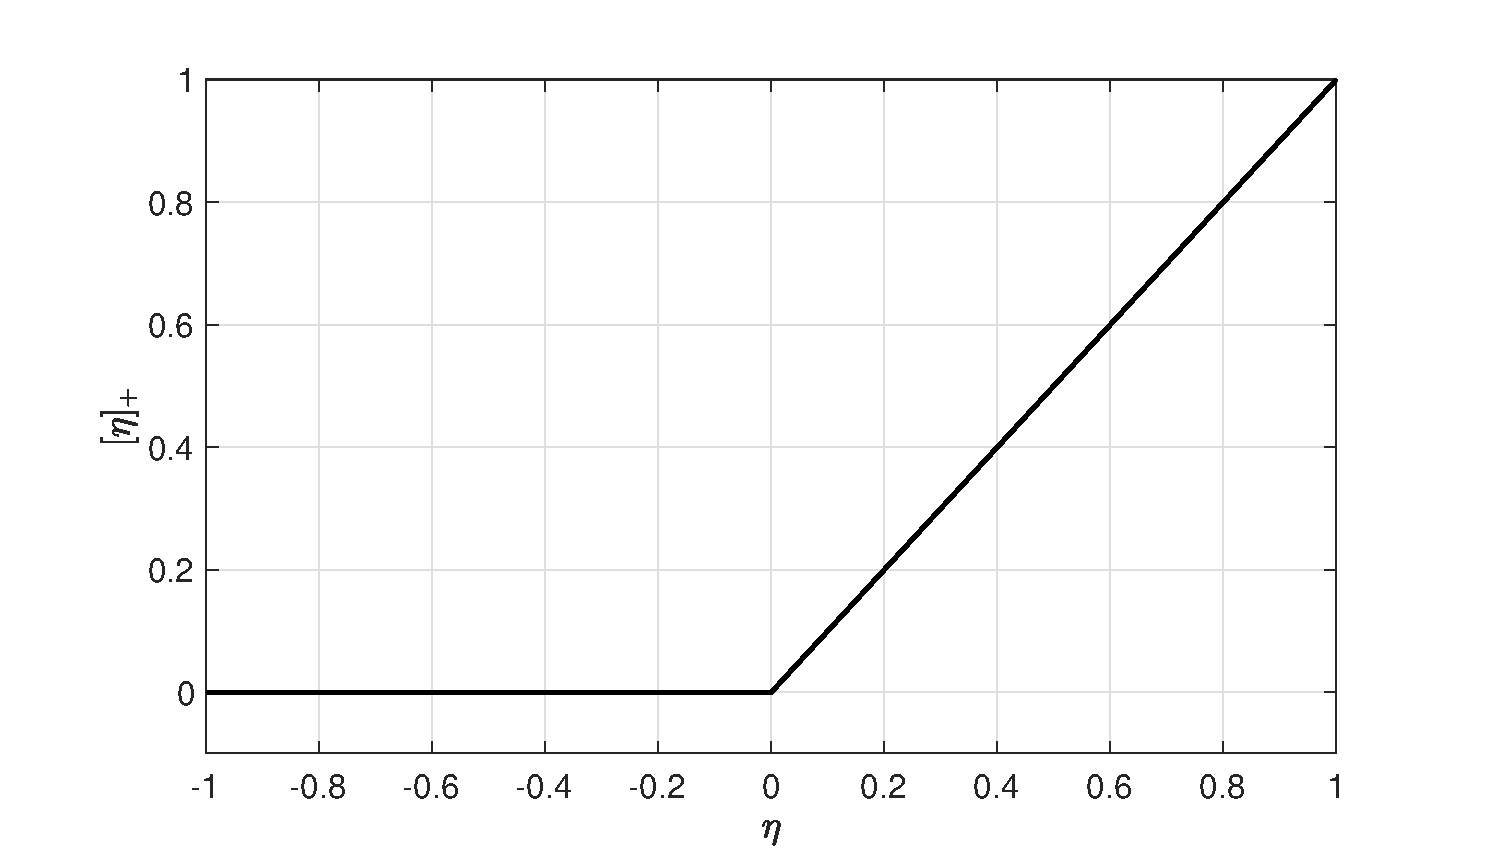
\includegraphics[width=0.6\columnwidth]{figures/interactions/eta.eps}}
\caption{\label{fig:eta}{A plot of $[\eta]_+$.}}
\end{figure}

\noindent The derivative of Eq. \eqref{eq:potential} with respect to $\eta$ is defined as 
\begin{equation}\label{eq:derivPotential}
    \phi'(\eta) = K[\eta]_+^{\alpha_\ctxt}
\end{equation}
and can then be used in the PDE at hand. 

The issue with this form of the collision potential, is that an iterative method, such as Newton-Raphson presented in Section \ref{sec:newtonRaphson} needs to be used in order to solve the system \cite{Ducceschi2021}.

\subsubsection{Quadratic form}
In \cite{Ducceschi2021}, the authors propose to rewrite the potential in Eq. \eqref{eq:derivPotential} in a quadratic form. Using the chain rule and  $\psi = \psi(\eta)$, Eq. \eqref{eq:derivPotential} can be rewritten as
\begin{equation}\label{eq:quadraticPotential}
    \phi'(\eta) = \psi\psi' \quad \text{where} \quad \psi = \sqrt{2\phi} \quad \text{and} \quad \psi' = \frac{\dot{\psi}}{\dot{\eta}}\ ,
\end{equation}
where a dot denotes a single derivative with respect to time. 

This form of the potential can be discretised to a FD scheme that can be solved explicitly. This process will be shown below, using an example of the simple mass-barrier collision. 

\section{The mass -- rigid barrier collision}\label{sec:massRigidBarrier}
As a test case, the simplest collision case -- a mass colliding with a rigid barrier -- is presented here. Consider a mass at location $u = u(t)$ (in m) colliding with a barrier at location $b$ (in m).

If the barrier is placed above the mass, the force it exerts on the mass will be negative and its system would be described as
\begin{equation}\label{eq:massBarrierPre}
    M\ddot u = -\psi\psi',
\end{equation}
with mass $M$ (in kg) and $\psi = \psi(\eta)$ and $\psi'$ are as defined in Eq. \eqref{eq:quadraticPotential} with $\eta = \eta(t) = u(t) - b$. 

Looking towards the discretisation the mass-barrier collision, one could rewrite Eq. \eqref{eq:massBarrierPre} to the following system of equations
\begin{subequations}\label{eq:massBarrier}
    \begin{align}
        M\ddot u &= -\psi g,\label{eq:massBarrierPDE1}\\
        \dot\psi &= g \dot\eta,\label{eq:massBarrierPDE2}\\
        \eta(t) &= u(t) - b,\label{eq:massBarrierPDE3}
    \end{align}
\end{subequations} 
where $g = \psi'$.

\subsubsection{Location of objects}
As explained in Chapter \ref{ch:connections}, it is important to consider whether an object is located `above' or `below' the other, 

% Notice that 
% it is important to keep in mind the relative location of the colliding objects, i.e., whether one object is `above' or `below' an other. 
or, which has a more positive or negative displacement than the other object. A mass with a displacement of $0.01$ m will thus be `above' a barrier with a displacement of $-0.05$ m. Along these lines, a positive force acting on an element will accelerate it upwards and a negative force will accelerate it downwards.

The relative location of the two colliding objects will affect two things in \eqref{eq:massBarrier}.
Firstly, the location of the object determines the direction of the collision force, i.e., the sign of the right-hand side in system \eqref{eq:massBarrierPDE1}. In this case, the barrier is placed above the mass, and will exert a downwards (negative) force on the mass. If the barrier was placed below the mass, the opposite would have applied.
Secondly, the definition of $\eta$ in \eqref{eq:massBarrierPDE3} is affected by the relative location of the objects. The collision potential in Eq \eqref{eq:potential} is only non-zero when $\eta$ is positive. If the barrier is placed above the mass, $u(t)-b$ will be positive on collision. It is thus important to remember that $\eta$ should be defined as the element above subtracted from the element below.\todo{This might need to be moved to the previous chapter. At least highlight the difference between a ``pushing'' collision and a ``pulling'' connection}

\subsection{Discrete time}
Before discretising system \eqref{eq:massBarrier} in full, the discrete approximation to the collision potential will be elaborated on.
Following \cite{Ducceschi2021}, $\psi$ is placed on an interleaved temporal grid using
\begin{equation}
    \psi^{n-1/2} = \mu_{t-}\psi^n,
\end{equation} 
where the interleaved temporal grid is used here as it results in energy conservation in discrete time as will be shown below. Approximations to $\psi$ and $g$ in Eq. \eqref{eq:massBarrier} can then be made as 
\begin{equation}
    \psi \approxeq \mtp \psi^{n-1/2}
\end{equation}
and 
\begin{equation}\label{eq:approxPsi}
    g \approxeq g^n = \frac{\delta_{t+}\psi^{n-1/2}}{\delta_{t\cdot}\eta^n} ,
\end{equation}
respectively. Notice that applying a first-order difference operator to a grid function on an interleaved grid is second-order accurate.\footnote{$\ \dtp \psi^{n-1/2}\ \overset{\text{Eq. \eqref{eq:approxPsi}}}{=}\ \dtp \mtm \psi^n\ \overset{\text{Eq. \eqref{eq:identity2}}}{=}\  \dtd \psi^n$ which is second-order accurate (see Section \ref{sec:FDoperators}).}
The result of the approximation to in Eq. \eqref{eq:approxPsi} allows $\psi$ to be treated as an independent time series:
\begin{equation}
    \dtp \psi^{n-1/2} = g^n \dtd \eta^n.
\end{equation}
With the above approximations in place, system \eqref{eq:massBarrier} can be discretised and yields the following system of equations: 
\begin{subequations}\label{eq:massBarrierSystem}
    \begin{align}
        M\dtt \un &= -\left(\mtp\psi^{n-1/2}\right)g^n,\label{eq:massBarrierSystem1}\\
        \dtp \psi^{n-1/2} &= g^n \dtd \eta^n,\label{eq:massBarrierSystem2}\\ 
        \eta^n &= \un - b.\label{eq:massBarrierSystem3}
    \end{align}
\end{subequations}


\subsubsection{An explicit definition for $g^n$}
To be able to calculate $\psi^{n+1/2}$ and $u^{n+1}$ in system \eqref{eq:massBarrierSystem} explicitly, a definition for $g^n$ only based on known values must be found. As $g^n \approxeq \psi'$ as per Eq. \eqref{eq:approxPsi}, the derivative can be computed analytically according to 
\begin{equation}
    g^n = \psi'\bigg\rvert_{\eta=\eta^n} \quad \overset{\text{Eq. \eqref{eq:quadraticPotential}}}{=}\quad  \frac{\phi'}{\sqrt{2\phi}}\bigg\rvert_{\eta=\eta^n}.
\end{equation}
Recalling \eqref{eq:derivPotential} and \eqref{eq:potential}, this can conveniently be rewritten to
\begin{equation}\label{eq:gn}
    g^n = \frac{K[\eta^n]_+^\alpha}{\sqrt{\frac{2K}{\alpha+1}[\eta^n]_+^{\alpha+1}}}=K\sqrt{\frac{\alpha+1}{2K}}[\eta^n]_+^\alpha[\eta^n]_+^{\frac{-(\alpha+1)}{2}}=\sqrt{\frac{K(\alpha+1)}{2}}[\eta^n]_+^{\frac{\alpha-1}{2}}\ .
\end{equation}
For implementation purposes, one can expand the $[\cdot]_+$ operator as the following (equivalent) condition:
\begin{subnumcases}{ \label{eq:gDefOld} g^n =}
    \sqrt{\frac{K_\text{c}(\alpha_\text{c}+1)}{2}}\cdot(\eta^n)^{\frac{\alpha_\text{c}-1}{2}}
    & if $\eta^n \geq 0$ \label{eq:collCorr1Old}\\
    0, & $\text{if } \eta^n < 0$\label{eq:collCorr2Old}
\end{subnumcases}
This implementation is the one presented in \cite{Ducceschi2019}, but exhibited spurious oscillations and `sticking' behaviour. This is due to the possibility of negative forces for positive penetrations due to the discontinuity in the definition for $g^n$ at $\eta^n = 0$.

In \cite{Ducceschi2021}, the definition for $g^n$ in \eqref{eq:gDefOld} is extended, starting out by using an implicit equation for $g^n$ by directly discretising Eq. \eqref{eq:approxPsi}
\begin{equation}\label{eq:gImp}
    g_\text{imp}^n = 2\frac{\psi^{n+1/2} - \psi^{n-1/2}}{\eta^{n+1} - \eta^{n-1}}.
\end{equation}
If there is, however, no collision at $n+1/2$, $\psi^{n+1/2} = 0$ and Eq. \eqref{eq:gImp} reduces to
\begin{equation*}
    g_\text{imp}^n = -2\frac{\psi^{n-1/2}}{\eta^{n+1} - \eta^{n-1}}.
\end{equation*}
Furthermore, due to the fact that there is no collision, $\eta^{n+1}$ can be calculated according to $\eta^{n+1} = \eta^\star = u^\star - b$ where $u^\star$ is the value of $u^{n+1}$ calculated using the scheme in Eq. \eqref{eq:massBarrierSystem1} without the collision force (as done in Chapter \ref{ch:connections}). Expanding Eq. \eqref{eq:massBarrierSystem1} without the collision force yields  
\begin{equation*}
    \frac{M}{k^2}\left(u^\star - 2\un + u^{n-1}\right) = 0 \quad \Longrightarrow \quad u^\star = 2u^n - u^{n-1}.
\end{equation*}
Thus, if there is no collision, $g^n_\text{imp}$ can now be explicitly calculated from known values and be used in the definition for $g^n$ in Eq. \eqref{eq:gDefOld} according to \cite{Ducceschi2021}
\begin{subnumcases}{ \label{eq:gDef} g^n =}
    \kappa\sqrt{\frac{K_\text{c}(\alpha_\text{c}+1)}{2}}\cdot(\eta^n)^{\frac{\alpha_\text{c}-1}{2}}
    & if $\eta^n \geq 0,$ \label{eq:collCorr1}\\
    -2 \frac{\psi^{n-1/2}}{\eta^\star-\eta^{n-1}} & if $\eta^n < 0\ \text{ and } \ \eta^{\star} \neq \eta^{n-1},$\label{eq:collCorr2}\\
    0, & $\text{if } \eta^n < 0\ \text{ and } \ \eta^{\star} = \eta^{n-1}.\qquad$\label{eq:collCorr3}
\end{subnumcases}
%
Here, $\kappa = 1$ if $\psi^{n-1/2} \geq 0$, otherwise $\kappa = -1$ and aims to resolve the `sticking' behaviour by forcing an outwardly-directed force at all times. As was done in paper \citeP[H], \eqref{eq:collCorr3} has been added to the definition of $g$ from \cite{Ducceschi2021} to prevent a division by 0 in \eqref{eq:collCorr2}. 

This definition for $g^n$ does not exhibit the spurious oscillations that the old definition in Eq. \eqref{eq:gDefOld} did, and can still be explicitly calculated from known values of the system. 

\subsection{Solving the system}\label{sec:solvingMassBarrier}
To implement the system in Eq. \eqref{eq:massBarrierSystem}, the equations need to be slightly rewritten. Using identity \eqref{eq:identity3}, $\mtp \psi^{n-1/2}$ can be rewritten to
\begin{equation*}
    \mu_{t+}\psi^{n-1/2} = \frac{k}{2}\delta_{t+}\psi^{n-1/2} + \psi^{n-1/2}.
\end{equation*}
Then, substituting \eqref{eq:massBarrierSystem2} into this yields
\begin{equation}\nonumber
    \mu_{t+}\psi^{n-1/2} = \frac{k}{2}g^n\delta_{t\cdot}\eta^n + \psi^{n-1/2},
\end{equation}
and inserting this into \eqref{eq:massBarrierSystem1} yields
\begin{equation}\label{eq:substitutionFDS}
    M\delta_{tt}u^n = -\Big(\frac{k}{2}g^n\delta_{t\cdot}\eta^n + \psi^{n-1/2}\Big)g^n\ .
\end{equation}
As the position of barrier $b$ is static, the following is true:
\begin{equation}\label{eq:derEtaEqDerU}
    \frac{d\eta}{dt} = \frac{d}{dt}\Big(u - b\Big)\quad \Longrightarrow \quad \delta_{t\cdot}\eta^n = \delta_{t\cdot}u^n,
\end{equation}
i.e., the time derivative of $\eta$ equals the time derivative of $u$.\footnote{Note that if the barrier was placed underneath the mass, making \eqref{eq:massBarrierSystem3} $\eta^n = b-u^n$, this would result in $\delta_{t_\cdot}\eta^n = -\delta_{t\cdot}u^n$.} Now \eqref{eq:substitutionFDS} can be solved explicitly as $u^{n+1}$ is the only unknown in the system
\begin{equation}
    \bigg(\frac{M}{k^2} + \frac{(g^n)^2}{4}\bigg)u^{n+1} = \frac{M}{k^2}(2u^n-u^{n-1})+\frac{(g^n)^2}{4}u^{n-1}-\psi^{n-1/2}g^n\ ,
\end{equation}
and can be solved by a simple division. 

Finally, $u^{n+1}$ can be used to calculate $\eta^{n+1}$ can be calculated using \eqref{eq:massBarrierSystem3} at $n+1$:
\begin{equation}\label{eq:etaNPlus1}
    \eta^{n+1} = u^{n+1}-b,
\end{equation}
which is used to calculate $\psi^{n+1/2}$ by expanding and rewriting \eqref{eq:massBarrierSystem2} to
\begin{equation}\label{eq:psiNPlusHalf}
    \psi^{n+1/2} = \psi^{n-1/2} + \frac{\eta^{n+1} - \eta^{n-1}}{2}\ .
\end{equation}

\subsection{Energy analysis}
To prove that the collision term does not add any additional energy into the system (retaining passivity) and that it does not add additional constraints on the stability of the system, the energy analysis techniques presented in Section \ref{sec:energyAnalysis} can be used. Notice that for brevity, the steps presented Section \ref{sec:energyAnalysis} will not explicitly be followed.

Multiplying Eq. \eqref{eq:massBarrierSystem1} by $(\dtd \un)$ yields 
\begin{equation*}
    \dtp \h  = -\left(\mtp\psi^{n-1/2}\right)g^n (\dtd \un)
\end{equation*}
where
\begin{equation}
    \h = \frac{M}{2}(\dtm\un)^2
\end{equation}
(see Eq. \eqref{eq:energyBalanceMassSpring}). Expanding $g^n$ yields 
\begin{align*}
    \dtp \h  &= -\left(\mtp\psi^{n-1/2}\right)\frac{\dtp \psi^{n-1/2}}{\dtd \eta^n}(\dtd \un)\\
    \xLeftrightarrow{\mystrut\ \text{Eq. \eqref{eq:derEtaEqDerU}}} \qquad & = -\left(\mtp\psi^{n-1/2}\right)\dtp \psi^{n-1/2},
\end{align*}
which, using identity \eqref{eq:prodIdentity3} can be rewritten to 
\begin{equation}
    \dtp(\h + \h_\ctxt) = 0,
\end{equation}
with collision energy
\begin{equation}\label{eq:collisionEnergy}
    \h_\ctxt = \frac{(\psi^{n-1/2})^2}{2}.
\end{equation}
Recall that in order for a scheme to be passive, its energy must be non-negative. The fact that $\psi$ is squared proves passivity for the system in \eqref{eq:massBarrierSystem}.

\section{Mass-spring -- string collision}\label{sec:massString}
The mass-spring -- string collision is slightly trickier than the mass -- rigid barrier collision, as there are two moving components rather than one. This system is chosen as an example as it has the interesting use-case of fretting a string to change the pitch, modelling the fretting finger as a mass.

Consider a lossless stiff string of length $L$, its transverse displacement described by $u = u(x,t)$ (in m) and defined over $x\in \D$ with domain $\D = [0, L]$. The mass with displacement $w = w(t)$ (in m) will model the fretting finger. The PDE for the stiff string and its parameter definitions can be found in Eq. \eqref{eq:stiffStringPDENoLosses} and for the mass-spring system in Eq. \eqref{eq:massSpringPDE}. Placing the string above the mass, the following system emerges:
\begin{subequations}\label{eq:massStringPDE}
\begin{align}   
    \rho A \ptt u & =T\pxx u - EI\pxxxx u + \delta(x-x_\text{m}) \psi g \label{eq:massStringPDE1}\\
    M \ddot w &=-Kw - \psi g\label{eq:massStringPDE2}\\
    \dot\psi &= g \dot\eta,\label{eq:massStringPDE3}\\
    \eta(t) &= w(t) - u(x_\text{m}, t),\label{eq:massStringPDE4}
\end{align}
\end{subequations}
where spatial Dirac delta function $\delta(x-x_\text{m})$ localises the mass (finger) along the string at location $x_\text{m} \in \D$. Furthermore $\psi = \psi(\eta)$ and $g=\psi'$ and are as defined in Eq. \eqref{eq:quadraticPotential}. 

Discretising system \eqref{eq:massStringPDE}, with the collision discretised according to the process explained in Section \ref{sec:massRigidBarrier}, yields
\begin{subequations}
    \begin{align}   
        \rho A \delta_{tt}u^n_l & =T\delta_{xx}u^n_l - EI\delta_{xxxx}u_l^n + J_l(x_\text{m}) \big(\mu_{t+}\psi^{n-1/2}\big)g^n, \label{eq:massString1}\\
        M \delta_{tt}w^n &=-Kw^n - \big(\mu_{t+}\psi^{n-1/2}\big)g^n,\label{eq:massString2}\\
        \delta_{t+}\psi^{n-1/2} &= g^n\delta_{t\cdot}\eta^n,\label{eq:massString3}\\
        \eta^n &= w^n - I_l(x_\text{m})\uln,\label{eq:massString4}
    \end{align}
\end{subequations}
where spreading and interpolation operators $I_l(x_\text{m})$ and $J_l(x_\text{m})$ are as defined in Section \ref{sec:interpolationSpreading} (the order is not specified here). Following the same process as in Section \ref{sec:solvingMassBarrier}, Eqs. \eqref{eq:massString1} and \eqref{eq:massString2} can be rewritten to 
\begin{subequations}\label{eq:massStringComb}
    \begin{align}
        \rho A \delta_{tt}u^n_l & =T\delta_{xx}u^n_l - EI\delta_{xxxx}u_l^n + J_l(x_\text{m}) \left(\frac{k}{2}g^n\delta_{t\cdot}\eta^n + \psi^{n-1/2}\right)g^n,\label{eq:massStringComb1}\\
        M \delta_{tt}w^n &=-Kw^n - \left(\frac{k}{2}g^n\delta_{t\cdot}\eta^n + \psi^{n-1/2}\right)g^n,\label{eq:massStringComb2}
    \end{align}
\end{subequations}
which can be used as a starting point for solving the system.

\subsection{Solving the system}
As the colliding objects are both moving, Eq. \eqref{eq:derEtaEqDerU} is not valid anymore and another strategy needs to be used.
One can start to solve the system by isolating the string at the collision location $x_\text{m}$ by taking an inner product of Eq. \eqref{eq:massStringComb1} with $J_l(x_\text{m})$. Using identity \eqref{eq:identityIJ} and dividing all terms by $\rho A$ yields
\begin{align*}
    \delta_{tt}I_l(x_\text{m})u^n_l =c^2I_l(x_\text{m})\delta_{xx}u^n_l &- \kappa^2I_l(x_\text{m})\delta_{xxxx}u_l^n \\
    &\quad + \frac{\lVert J_l(x_\text{m})\rVert^2_\D}{\rho A} \left(\frac{k}{2}g^n\delta_{t\cdot}\eta^n + \psi^{n-1/2}\right)g^n.
\end{align*}
with $c = \sqrt{T/\rho A}$ and $\kappa = \sqrt{EI/\rho A}$. Expanding the temporal FD operators yields 
\begin{align*}
    I_l(x_\text{m})u_l^{n+1} &= u^\star+ \underbrace{\frac{\lVert J_l(x_\text{m})\rVert^2_\D k^2}{\rho A}}_{\mathfrak{J}_l} \left(\frac{(g^n)^2}{4}\left(\eta^{n+1}-\eta^{n-1}\right) + \psi^{n-1/2}g^n\right),
\end{align*}
where 
\begin{equation*}
    u^\star = I_l(x_\text{m})(2u_l^n -u_l^{n-1}) + c^2k^2I_l(x_\text{m})\delta_{xx}\uln- \kappa^2k^2I_l(x_\text{m})\delta_{xxxx}\uln
\end{equation*}
is the result of the update equation of the string at $x_\text{m}$ without the collision term. Then, Eq. \eqref{eq:massString4} at $n+1$, which is $\eta^{n+1} = w^{n+1} - I(x_\text{m})u_l^{n+1}$, can be substituted, which results in
\begin{equation}\label{eq:expandedMassString1}
    \begin{aligned}
    \left(1 + \mathfrak{J}_l\frac{(g^n)^2}{4}\right)I_l(x_\text{m})u_l^{n+1} - \mathfrak{J}_l&\frac{(g^n)^2}{4} w^{n+1}= u^\star\\
    & + \mathfrak{J}_l \left(-\frac{(g^n)^2}{4}\eta^{n-1} + \psi^{n-1/2}g^n\right).
    \end{aligned}
\end{equation}
    
Performing this same process on the FD scheme of the mass in Eq. \eqref{eq:massStringComb2} yields
\begin{equation}\label{eq:expandedMassString2}
    \begin{aligned}
    -\frac{(g^n)^2 k^2}{4M} I_l(x_\text{m})u_l^{n+1} + &\left(1 + \frac{(g^n)^2 k^2}{4M}\right)w^{n+1} = w^\star\\
    & - \frac{k^2}{M} \left(-\frac{(g^n)^2}{4}\eta^{n-1} + \psi^{n-1/2}g^n\right),
    \end{aligned}
\end{equation}
where 
\begin{equation*}
    w^\star = 2w^n - w^{n-1} - \frac{Kk^2}{M}w^n
\end{equation*}
is again the result of the update equation of the mass without the collision term.
Equations \eqref{eq:expandedMassString1} and \eqref{eq:expandedMassString2} can be treated as a system of linear equations (see Section \ref{sec:linearEquations}) with unknowns $I_l(x_\text{m})u^{n+1}$ and $w^{n+1}$. Writing the aforementioned equations in matrix form yields
\begin{align}
    \begin{bmatrix}
            I_l(x_\text{m})u^{n+1}_l\\
            w^{n+1}
        \end{bmatrix}
        = 
        \mathbf{A}^{-1}\mathbf{v}
    \end{align}
    where
    \begin{equation}
    \begin{gathered}
    \mathbf{A} = 
        \begin{bmatrix}
            \left(1 + \mathfrak{J}_l\frac{(g^n)^2}{4}\right) & -\mathfrak{J}_l\frac{(g^n)^2}{4}\\
            -\frac{(g^n)^2 k^2}{4M} &\left(1 + \frac{(g^n)^2 k^2}{4M}\right)
        \end{bmatrix}
        \quad \text{and}\\
        \mathbf{v} = 
        \begin{bmatrix}
            u^\star + \mathfrak{J}_l \left(-\frac{(g^n)^2}{4}\eta^{n-1} + \psi^{n-1/2}g^n\right)\\
            w^\star- \frac{k^2}{M} \left(-\frac{(g^n)^2}{4}\eta^{n-1} + \psi^{n-1/2}g^n\right)
        \end{bmatrix}.
        \nonumber
    \end{gathered}
\end{equation}
From this, $\eta^{n+1}$ can be calculated, and can consequently be applied to the string and mass in system \eqref{eq:massStringComb}.

\subsection{Energy analysis}
This section follows Section \ref{sec:energyAnalysis} without explicitly following the steps for brevity. 

One can obtain the energy of the stiff string FD scheme in Eq. \eqref{eq:massString1} by taking the inner product of scheme by $\dtd \uln$ over domain $\D$ to obtain 
\begin{equation}\label{eq:rOCEnergyString}
    \dtp \h_\text{s} = \left\langle (\dtd \uln), J_l(x_\text{m})\left(\mtp \psi^{n-1/2}\right)g^n\right\rangle_\D
\end{equation}
where (see Eq. \eqref{eq:energyBalanceStiffString})
\begin{equation*}
    \begin{gathered}
        \h_\text{s} = \t_\text{s} + \v_\text{s}, \qwiq \t_\text{s} = \frac{\rho A}{2}\lVert\dtm \uln\rVert^2_d,\quad \text{and} \\
        \v_\text{s} = \frac{T}{2}\langle\dxp\uln, e_{t-}\dxp\uln\rangle_{\underline{d}} + \frac{EI}{2}\langle\dxx\uln, e_{t-}\dxx\uln\rangle_{\overline{\underline{d}}}\ .
    \end{gathered}
\end{equation*}
Energy analysis for the mass in Eq. \eqref{eq:massString2} can be done by simply multiplying the scheme by $\dtd w^n$ to get 
\begin{equation}\label{eq:rOCEnergyMass}
    \dtp \h_\text{m} = -(\dtd w^n)\left(\mtp \psi^{n-1/2}\right)g^n,
\end{equation}
where (see Eq. \eqref{eq:energyBalanceMassSpring})
\begin{equation*}
    \h_\text{m} = \t_\text{m} + \v_\text{m}, \qwiq \t_\text{m} = \frac{M}{2}(\dtm w^n)^2, \qaq \v_\text{m} = \frac{K}{2}w^n e_{t-}w^n.
\end{equation*}
The total energy in the system is the addition of Eqs. \eqref{eq:rOCEnergyString} and \eqref{eq:rOCEnergyMass}, which, using identity \eqref{eq:identityIJ} for the former, can be written as:
\begin{align*}
    \dtp(\h_\text{s} + \h_\text{m}) &= \Big(I_l(x_\text{m})(\dtd \uln) - (\dtd w^n)\Big)\left(\mtp \psi^{n-1/2}\right)g^n,\\
    &= \underbrace{\dtd\left(I_l(x_\text{m})\uln - w^n\right)}_{-\dtd \eta^n}\left(\mtp \psi^{n-1/2}\right)g^n.
\end{align*}
Then, expanding $g^n$ according to Eq. \eqref{eq:approxPsi} yields 
\begin{align*}
    \dtp(\h_\text{s} + \h_\text{m}) &= - \dtd\eta^n\left(\mtp \psi^{n-1/2}\right)\frac{\delta_{t+}\psi^{n-1/2}}{\delta_{t\cdot}\eta^n}\\
    &= -\left(\mtp \psi^{n-1/2}\right)\delta_{t+}\psi^{n-1/2}
\end{align*}
and finally, using identity \eqref{eq:prodIdentity3}, can be rewritten as
\begin{equation}
    \dtp(\h_\text{s} + \h_\text{m} + \h_\text{c}) = 0,
\end{equation}
with collision energy
\begin{equation*}
    \h_\text{c} = \frac{(\psi^{n-1/2})^2}{2}.
\end{equation*}
Again, the fact that $\psi$ is squared here, means that $\h_\text{c}$ is non-negative, and proves passivity of the system. 

\section{Two-sided collision: A connection}\label{sec:twoSidedCollision}

% As an alternative to the method connections shown in Chapter \ref{ch:connections} showed ways to connect various resonators using techniques presented in \cite{theBible}. An alternative method to establish these connections can be devised using the methods presented in this chapter.
% 

Using the methods presented in this chapter, one could devise a two-sided collision and alter the collision potential in Eq. \eqref{eq:potential} to \cite{Bilbao2019}
\begin{equation}\label{eq:twoSidedPotential}
    \phi(\eta) = \frac{K}{\alpha_\ctxt+1}|\eta|^{\alpha_\ctxt+1},
\end{equation}
and taking its derivative with respect to $\eta$ yields
\begin{equation}
    \phi'(\eta) = \sgn(\eta)K|\eta|^{\alpha_\ctxt}.
\end{equation}
One can observe that, as opposed to the (one-sided) potential presented in Eq. \eqref{eq:potential}, the collision force will be non-zero, for both a positive and negative $\eta$. This two-sided collision can be used as a connection -- as an alternative to the connections presented in Chapter \ref{ch:connections} -- and has been used in papers \citeP[D] and \citeP[E] in combination with Eq. \eqref{eq:potential} to model the mechanics of the tromba marina. See Chapter \ref{ch:tromba} for more details.